\chapter{\textbf{Graphical representation in research}}


When presenting ideas that include references to data, it can be helpful to make the point using a graph or table. These visual methods can make the point much stronger than simply describing the data. Appropriate use of graphs is one way to enhance the message we are delivering.

\textbf{ Info graphics and data driven graphs}\cite {Shelley Fishel}

An info graphic (information graphic) is a representation of information in a graphic format designed to make the data easily understandable at a glance. People use info graphics to quickly communicate a message, to simplify the presentation of large amounts of data, to see data patterns and relationships, and to monitor changes in variables over time.
Info graphics include bar graphs, pie charts, histograms, line charts, tree diagrams, mind maps, Gantt charts, and network diagrams. Info graphics predate writing as a means of disseminating information. The process of creating info graphics is sometimes referred to as data visualization.
Some of the info graphs and data driven graphs are shown below

\begin{figure}
  % Requires \usepackage{graphicx}
  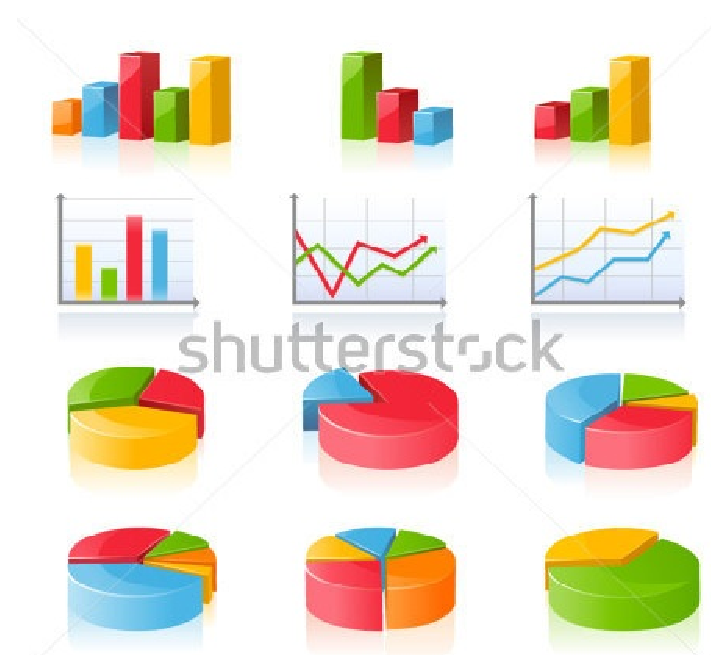
\includegraphics[width=4in]{figure1.eps} \cite  { Stephen Moffat}
  \caption {Example of Info graphs}\label{2.1} 
\end{figure} 
\textbf{Procedure for preparing info graph (Bar chart)}
\begin{enumerate}
  \item \textbf{Step 1: Draw the usual column chart}
  Let's take a column chart that shows number of new apartments constructed in the last 3 months in an area. The chart shows figures in thousands:
  \item \textbf{Step 2: Copy a relevant image}

 Choose a relevant image you want to fill in the columns. When you click on the image and press 'Ctrl+C', the picture gets copied to the clipboard. Let's take the image of a residential building to 'copy to clipboard art shows figures in thousands
  \item \textbf{Step 3: Select the columns and paste the image}
The next step is to click on the columns. When you click once, the entire series gets collected. When you click again only a single data point in the series gets selected. Let's select the series by clicking once on the chart columns:
Now press 'Ctrl+V' to paste the image.
\end{enumerate}


\begin{figure}
  % Requires \usepackage{graphicx}
  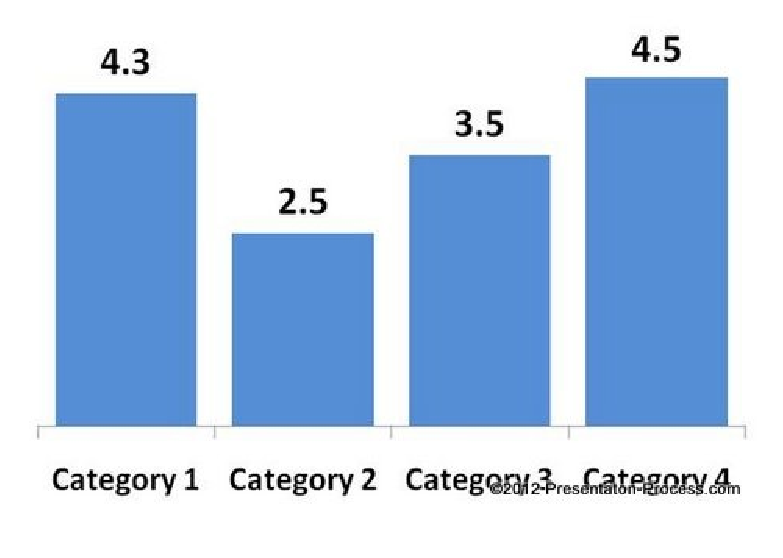
\includegraphics[width=4in]{figure2.eps} \cite {  Negriono}
  \caption {Column  chart}\label{3.2}
\end{figure}




     \begin{figure}
  % Requires \usepackage{graphicx}
  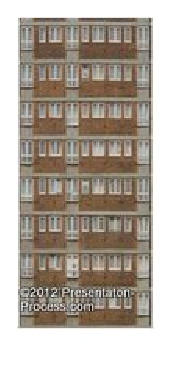
\includegraphics[width=1in]{figure3.eps}
  \caption {Column chart with clipboard art in it}\label{3.3} \cite {Anna and Bob}
\end{figure}




\begin{figure}
  % Requires \usepackage{graphicx}
  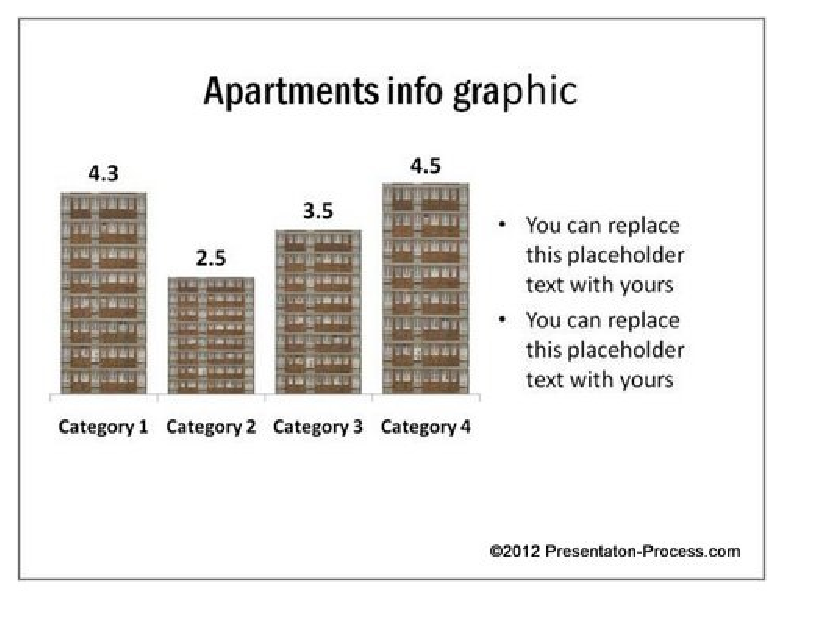
\includegraphics[width=2in]{figure4.eps} \cite {Anna and Bob}
  \caption {Image in Info Graph}\label{3.4}
\end{figure}




Availability of belief propagation algorithm in research papers shown by Bar graph.

\begin{itemize}
  \item CATOGORY 1(Springer) -.40
  \item CATOGORY 2(IEEE) -.50
  \item CATOGORY 3(Elsevier)-.60
\end{itemize}

\begin{figure}
  % Requires \usepackage{graphicx}
  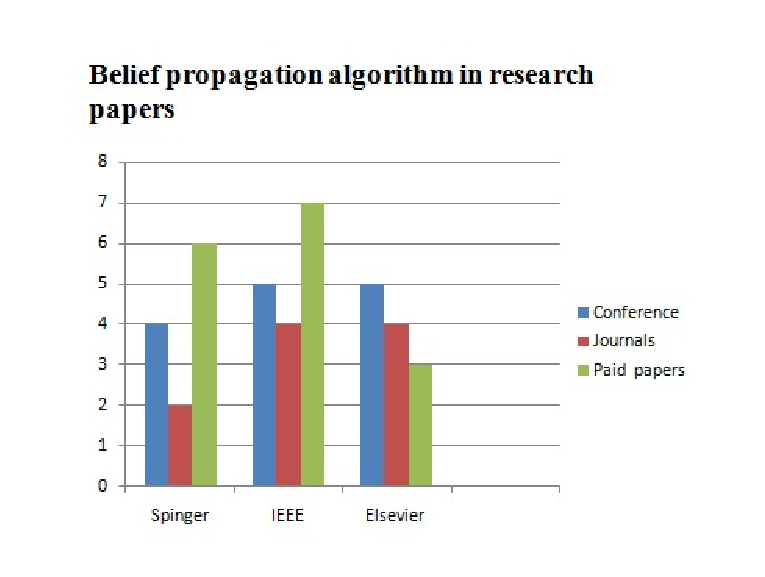
\includegraphics[width=2in]{figure5.eps}
  \caption {Representation of BP algorithm in column chart}\label{3.5}
\end{figure}






\textbf{3.1.2. PIE Graph}
The Pie chart is explained by considering an example of Application of Belief propagation

The Belief propagation algorithm is used in Code division multiple access (CDMA) -20%,
Image and Signal processing- 20%, low-density parity-check (LDPC)   Code -40% and
Artificial intelligence- 20%
%%%%%%%%%%%%%%%%%%%%%%%%%%%%%%%%%%%%%%%%%%%%%%

\textbf{Procedure to create a Pie Chart}
 \begin{itemize}
   \item Select the data from excel file
   \item On the Insert tab, in the Charts group, choose Pie, and select Pie
 \end{itemize}

 for e.g.: select data from A1:B4
\begin{figure}
  % Requires \usepackage{graphicx}
  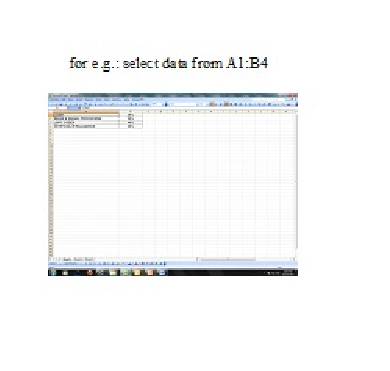
\includegraphics[width=2in]{figure6.eps} \cite { Stephen Moffat}
  \caption {select data from A1:B4}\label{3.6}
\end{figure}


Application of Belief propagation is shown by pie chart

\begin{figure}
  % Requires \usepackage{graphicx}
  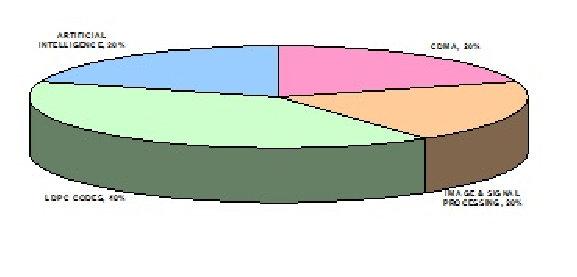
\includegraphics[width=2in]{figure7.eps}
  \caption {Application of Belief propagation}\label{3.7}
\end{figure}




\begin{itemize}
  \item Try not to use Clip Art (files of images that come free with software packages) that has seen in lots of other people's presentations: familiar images have less impact on an audience.
  \item Choose an appropriate quality for scanned images. Scan at 150 dpi for images where accurate color reproduction is not important and at 300 dpi for higher quality images
    \item Beware of images that take from the internet. They are generally of a very low quality and are likely to pixel ate (lose their smoothness) when you project them onto a large screen.
  \item Make sure graphics are relevant to text and not just decorative.
  \item Consider using graphics to replace text where an image would be easier to understand.
  \item Ensure that the images that use are simple and clear enough to be easily read at a distance. A small, overly complex and poor quality image will only frustrate audience.
  \item \textbf{Using animations and transitions}
Animating elements of slides and using Slide Transition are two of the most powerful features that PowerPoint offers. However, it is very easy to overdo use of these features and create a presentation where the animation distracts audience from the content of presentation
  \item Use animations to show progression. Animation is very effective at revealing a process one stage at a time.
  \item Be conservative. Make sure that any animation use serves a clear purpose (e.g. to introduce a new piece of information at an appropriate point). If cannot think of a reason to animate slide - don't do it!
\item Be consistent. Try to ensure that use similar types of animation for similar functions. For example, if text always drives in from the left it will be distracting if it suddenly appears from another direction or uses another animation technique.
\end{itemize}

\begin{figure}
  % Requires \usepackage{graphicx}
  
\includegraphics[width=2in]{figure8.eps} \cite  { Shelley Fishel}
  \caption {Application of BP in Pie chart}\label{3.8}
\end{figure}



MS Power Point allows you to easily include graphics in presentations, but while using graphics below listed points to be considered
	

\textbf{\textbf{3.2. Power point models in research}}

\textbf{Eye-catching PowerPoint Spiral Chart for research Process} \cite {Codeman Lisa}

The spiral chart diagram is as useful as it is beautiful. We can use the diagram anywhere we want to represent 'INPUT - Process- OUTPUT' cycle.


\begin{figure}
  % Requires \usepackage{graphicx}
  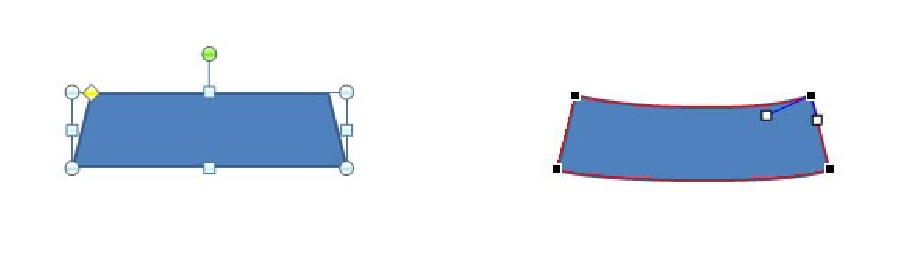
\includegraphics[width=4in]{figure9.eps} \cite {  Stephen Moffat}
  \caption {Sample of spiral chart}\label{3.9}
\end{figure}





\textbf{Procedure for preparing a Spiral Chart Diagram}
\begin{itemize}
  \item Design the initial shape for the Spiral Diagram
  \item Start designing a simple trapezium shape in Power Point.
  \item Editing the anchor points can convert the edges of the trapezium to curves so this will help to represent the spiral. Make sure to right click on the shape and then click on Edit Points.

  \item Now we can select the top and bottom edge and right click again to choose Curved Segment. \cite {Stephen Moffat}
\end{itemize}
.	
\begin{figure}
  % Requires \usepackage{graphicx}
  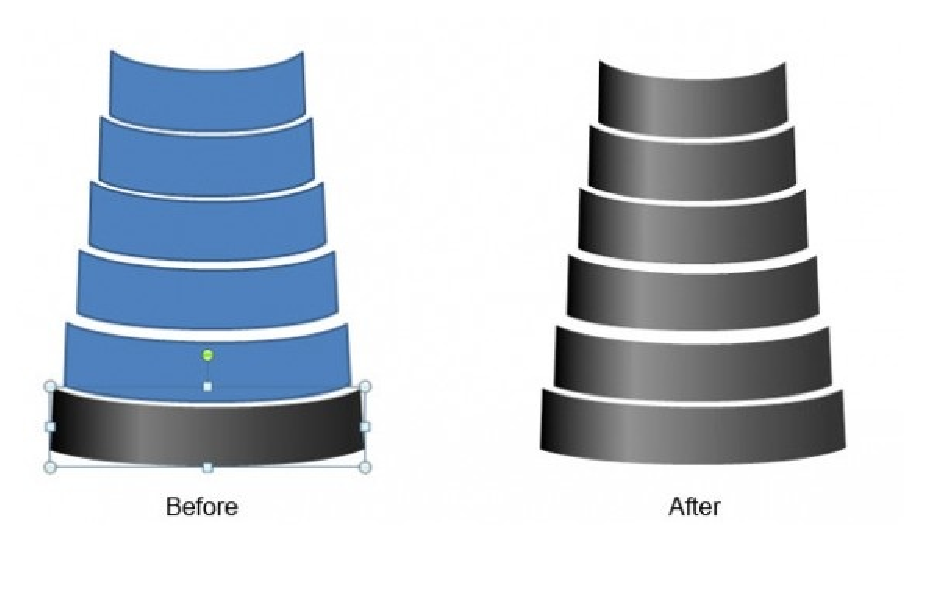
\includegraphics[width=2in]{figure10.eps} \cite { Stephen Moffat}
  \caption {Editing edges of the trapezium to curves}\label{3.10}
\end{figure}




	
We can copy and paste this multiple times and then use the useful tip to apply format painter multiple times.

\begin{figure}
  % Requires \usepackage{graphicx}
  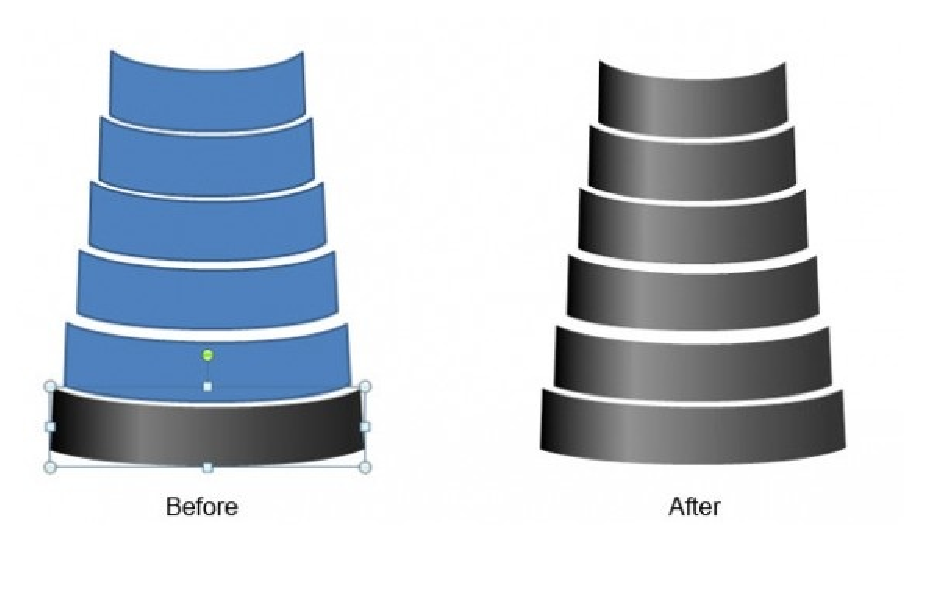
\includegraphics[width=2in]{figure10.eps}\cite { Stephen Moffat}
  \caption {Create the front of spiral diagram}\label{3.11}
\end{figure}




Create the front of spiral diagram

Now, we can replicate the shape multiple times. A quick tip for this is to keep the CTRL key pressed while you drag the shape to another position. Repeat this multiple times and reduce the shapes size to achieve the following design.


\begin{figure}
  % Requires \usepackage{graphicx}
  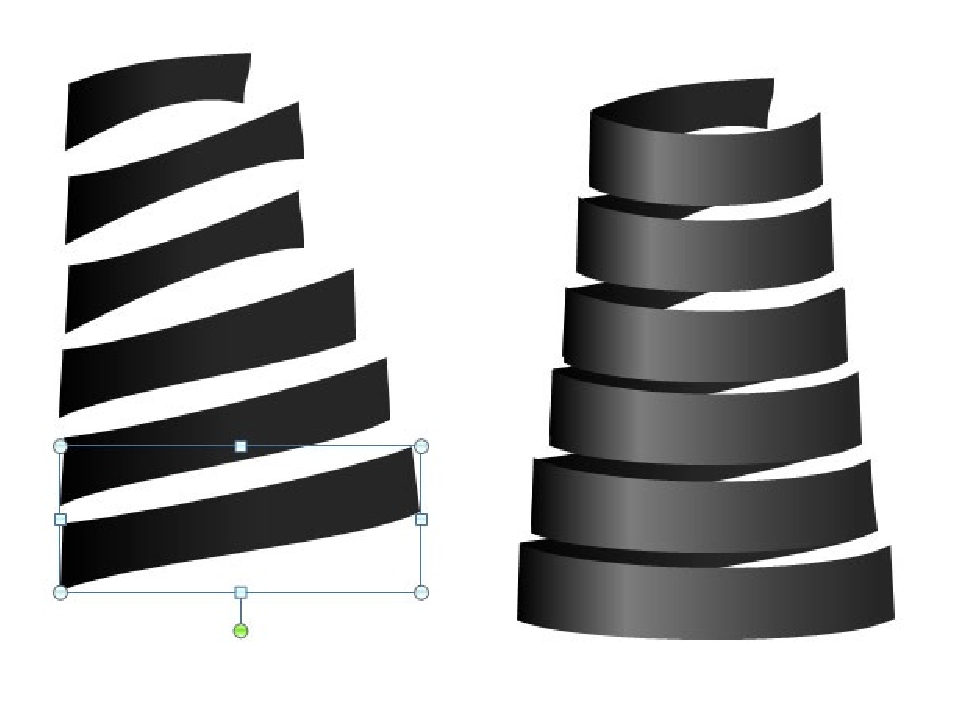
\includegraphics[width=2in]{figure12.eps}\cite { Stephen Moffat}
  \caption {Back of spiral diagram}\label{3.14}
\end{figure}
Create the back side
Now, add the shapes on the back of this spiral diagram. Below an example showing how these additional shapes will look. Of course it need to match with previous shapes and move the shapes to the back.
Then ready to wrap up the diagram and get this nice spiral chart in  MS Power Point. Add labels and text boxes around the spiral diagram to describe a process or other idea



















